\chapter{静态无向模型}
\label{chap:pgm-energy-models}

一排检测位置的状态通常不是彼此独立的：相邻位置可能共同过热，也可能因同一种测量干扰而同时出现异常。若已经知道每个位置的局部偏好和相邻位置的相容程度，怎样把这些信息组成整排状态的概率？如果温度读数已经给定，任务只剩下预测各位置的异常标签，又是否还需要解释这些读数本身怎样产生？

这两个问题共享局部势函数，却有不同的归一化对象。联合无向模型为所有建模变量的配置分配概率；条件无向模型固定输入，只比较可能的输出配置。第~\ref{chap:pgm-undirected}章已经建立无向分解与条件独立的联系，本章据此选择具体分布，考察哪些结构使推断可计算，以及增加潜变量、扩大势的作用域或改用神经参数化后，计算困难转移到了哪里。联合与条件是这里的主分类轴；观测或潜变量、成对或高阶势、固定特征或神经参数化都是可以交叉的属性，并非互斥的模型类别。

\section{无向模型的共同形式}
\label{sec:pgm-energy-models-common}

设无向图为$\mathcal{G}=(V,E)$，$d=|V|$，节点变量组成$\bm{X}=(X_1,\ldots,X_d)^\top$。若某个局部配置符合建模偏好，就给它较大的\term{势函数}（potential function）值；势表达的是相对相容程度，不要求其自身求和为$1$。以$\mathcal{C}$表示所用因子的作用域集合，每个$C\in\mathcal{C}$都是图中的一个团，不必是极大团。对严格正的势$\psi_{\bm{\theta},C}$，定义局部能量$E_{\bm{\theta},C}=-\log\psi_{\bm{\theta},C}$，便得到
\begin{equation}
  \begin{aligned}
    E_{\bm{\theta}}(\bm{x})
      &=\sum_{C\in\mathcal{C}}E_{\bm{\theta},C}(\bm{x}_C),\\
    p_{\bm{\theta}}(\bm{x})
      &=\frac{\prod_{C\in\mathcal{C}}
               \psi_{\bm{\theta},C}(\bm{x}_C)}
              {Z_{\bm{\theta}}}
        =\frac{\exp[-E_{\bm{\theta}}(\bm{x})]}{Z_{\bm{\theta}}},\\
    Z_{\bm{\theta}}
      &=\int \exp[-E_{\bm{\theta}}(\bm{u})]\,\mathrm{d}\mu(\bm{u}).
  \end{aligned}
  \label{eq:pgm-energy-models-joint}
\end{equation}
这里$\bm{\theta}$收集所有参数，$\mu$在离散空间上是计数测度，在连续空间上是指定的基准测度，通常为Lebesgue测度。\term{能量函数}（energy function）把局部偏好加起来，数值越小的配置具有越大的未归一化权重；\term{配分函数}（partition function）$Z_{\bm{\theta}}$则把所有配置的权重汇总，要求$0<Z_{\bm{\theta}}<\infty$。本章的能量是无量纲的对数权重，物理模型中的逆温度已吸收到参数里。

负能量$f_{\bm{\theta}}=-E_{\bm{\theta}}$也可作为得分，但它还不是对数概率；后者是$f_{\bm{\theta}}-\log Z_{\bm{\theta}}$。给能量加一个不依赖$\bm{x}$的常数，只会同时缩放分子与配分函数，不改变分布；把能量乘以一个正数则通常会改变分布的集中程度。比较同一个模型内两种配置时，配分函数约去：
\[
  \frac{p_{\bm{\theta}}(\bm{x})}{p_{\bm{\theta}}(\bm{x}')}
  =\exp\{E_{\bm{\theta}}(\bm{x}')-E_{\bm{\theta}}(\bm{x})\}.
\]
这使得能量差足以排序配置，却不足以给出某一配置的绝对概率。只修改一个局部势，也会改变$Z_{\bm{\theta}}$，进而改变其他配置的概率；局部参数正是通过这个总和与全局分布联系起来。

当输入$\bm{x}$已经给定、输出为$\bm{Y}$时，保留相同构造，但把求和或积分限制在输出空间：
\begin{equation}
  \begin{aligned}
    p_{\bm{\theta}}(\bm{y}\mid\bm{x})
      &=\frac{\exp[-E_{\bm{\theta}}(\bm{y},\bm{x})]}
              {Z_{\bm{\theta}}(\bm{x})},\\
    Z_{\bm{\theta}}(\bm{x})
      &=\int\exp[-E_{\bm{\theta}}(\bm{v},\bm{x})]
                  \,\mathrm{d}\mu_Y(\bm{v}).
  \end{aligned}
  \label{eq:pgm-energy-models-conditional}
\end{equation}
每个实际使用的输入都必须满足$0<Z_{\bm{\theta}}(\bm{x})<\infty$。这没有定义$p(\bm{x})$：输入之间可以有复杂依赖，模型不负责给它们分配生成概率。相应地，任意只依赖输入的附加能量$c(\bm{x})$都会约掉。图~\ref{fig:pgm-energy-models-normalization}强调了这一差别：条件无向模型中的输入可以影响多个势，但不参与本次归一化。

\begin{figure}[htbp]
  \centering
  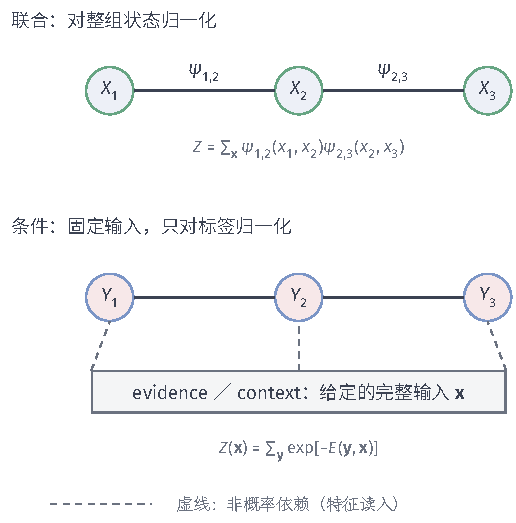
\includegraphics[width=\linewidth]{figures/03-models/03-probabilistic-graphical-models/tikz/pgm-energy-models-normalization/figure.pdf}
  \caption{相同的三节点相互作用可以用于联合或条件建模。上图对整组状态求和；下图用灰底框把$\bm{x}$明确标成evidence／context，只对标签$\bm{y}$求和。图内图例说明虚线是特征读入形成的非概率依赖，不是概率图中的有向生成边。}
  \label{fig:pgm-energy-models-normalization}
\end{figure}

有限离散状态、有限能量自动给出正且有限的配分函数。连续空间没有这一便利：$E(x)=-x^2$处处有定义，但$\int_{\mathbb{R}}e^{x^2}\,\mathrm{d}x$发散。若允许零势，可将对应能量记为$+\infty$来排除某些配置；此时须保留至少一个有正权重的离散配置，连续情形则须保留正测度的有效支持。零势不妨碍由分解推出Markov性质，但不能直接调用要求严格正性的反向分解定理。有关条件已在第~\ref{chap:pgm-undirected}章说明。

\section{联合能量模型}
\label{sec:pgm-energy-models-joint-models}

联合建模适合需要补全未知状态、计算多变量事件概率或生成整组配置的任务。下面从成对作用出发，分别改变变量是否可见、能量的函数形式和势的作用域。每次变化都保留式~\eqref{eq:pgm-energy-models-joint}，但可用的推断运算并不相同。

\subsection{观测变量成对模型}
\label{sec:pgm-energy-models-pairwise}

当每个位置只有两种状态时，可用$x_i\in\{-1,+1\}$表示。\term{Ising模型}（Ising model）用一个参数描述每个位置偏向哪种状态，再用一个参数描述每对相邻位置偏好同号还是异号：
\begin{equation}
  E_{\bm{\theta}}(\bm{x})
    =-\sum_{i\in V}b_ix_i
     -\sum_{\{i,j\}\in E}J_{i,j}x_ix_j.
  \label{eq:pgm-energy-models-ising}
\end{equation}
$b_i$称为\term{外场}（external field），正值偏好$+1$；$J_{i,j}$是\term{耦合参数}（coupling parameter），正值奖励同号，负值奖励异号。每条无向边只计算一次，且记$J_{i,j}=J_{j,i}$。无向耦合描述统计相互作用，不意味着干预一个节点会按该参数改变另一个节点。

固定其余节点后，含$x_i$的得分只有$x_i(b_i+\sum_{j\in N(i)}J_{i,j}x_j)$，其中$N(i)$是邻居集合。因此两种状态的权重比为$\exp[2(b_i+\sum_jJ_{i,j}x_j)]$，从而
\begin{equation}
  \begin{aligned}
    p_{\bm{\theta}}(X_i=+1\mid\bm{x}_{V\setminus\{i\}})
      &=\sigma\!\left(2b_i+
           2\sum_{j\in N(i)}J_{i,j}x_j\right),\\
    \sigma(u)&=\frac{1}{1+e^{-u}}.
  \end{aligned}
  \label{eq:pgm-energy-models-ising-conditional}
\end{equation}
只需邻居的状态便可计算满条件概率，但这不表示无边节点在未给定邻居时独立。

以三个相邻检测位置为教学例子，图为$1-2-3$，没有单点偏好，每条边的势在同号时为$3$、异号时为$1$。这些数值是人为设定的相容权重，不是测量频率。记相同相邻对的数量为
\[
  N_{=}(\bm{x})
   =\mathbf{1}\{x_1=x_2\}+\mathbf{1}\{x_2=x_3\}.
\]
选取能量$E_0(\bm{x})=-(\log3)N_{=}(\bm{x})$，联合权重为$3^{N_{=}(\bm{x})}$。由于$x_1$有两种选择，每个后继状态的权重和均为$3+1=4$，配分函数为$Z_0=2\times4\times4=32$。这是$J_{1,2}=J_{2,3}=(\log3)/2$的Ising模型，因为$\mathbf{1}\{x_i=x_j\}=(1+x_ix_j)/2$。不过，$E_0$比式~\eqref{eq:pgm-energy-models-ising}的零外场能量少一个常数$\log3$，所以按后者计算的配分函数为$32/3$；分布相同，配分函数的数值不必相同。

在这个对称链上，给定前一个位置，后一个位置与它同号的概率为$3/4$，异号的概率为$1/4$。两端同号可以经过两次保持或两次改变，因此
\[
  p(X_3=X_1\mid X_1)
    =(3/4)^2+(1/4)^2=\frac58.
\]
每个节点的边缘概率都是$1/2$，于是$\mathbb{E}[X_1X_3]=2(5/8)-1=1/4$。虽然$1$与$3$没有直接相连，它们仍相关；给定$X_2$后才独立。对同样的更长零外场链，每条边使条件均值乘以$1/2$，相隔$r$条边的相关为$(1/2)^r$。局部相互作用可以沿路径传递，传递强度依赖参数，而非只取决于是否相邻。

若每个位置有$K>2$个类别，类别编号的乘积不再有自然含义。\term{Potts模型}（Potts model）以“类别是否相同”表达相容性，对$x_i\in\{1,\ldots,K\}$取
\begin{equation}
  E_{\bm{\theta}}(\bm{x})
   =-\sum_i b_i(x_i)
    -\sum_{\{i,j\}\in E}J_{i,j}\mathbf{1}\{x_i=x_j\}.
  \label{eq:pgm-energy-models-potts}
\end{equation}
$b_i(k)$是位置$i$对类别$k$的偏好。固定邻居后，对各候选类别计算权重
\[
  w_i(k)=\exp\left\{
    b_i(k)+\sum_{j\in N(i)}J_{i,j}\mathbf{1}\{k=x_j\}
  \right\},
\]
再除以$\sum_{\ell=1}^K w_i(\ell)$，便得到节点$i$的满条件概率。所有类别相等与否共用一个边参数，这是有意施加的限制；若某两种不同类别特别相容，就需要一般的$K\times K$边势表。二类Potts在重新编码后与Ising相容，但耦合系数相差上面的$1/2$，不能不经转换直接比较。

学习这两类模型时，一条完整记录给出节点取值和边上的乘积或同类指示量。固定图后，最大似然要求这些经验统计量与模型期望匹配；例如Ising的$J_{i,j}$更新使用经验$x_ix_j$减去模型的$\mathbb{E}[X_iX_j]$。通用梯度与替代准则见第~\ref{chap:pgm-parameter-learning}章。模型特有的便利是式~\eqref{eq:pgm-energy-models-ising-conditional}可直接用于Gibbs更新或伪似然拟合；限制则是邻居之间强耦合时，单点更新可能很难从一种整体配置走到另一种。

在树上，用一般稠密边势计算配分函数和边缘需要$O(dK^2)$运算，特殊势还能进一步化简。一般图的精确消元则受诱导宽度控制，不能因为每个原始因子只含两个变量，就断言整个计算是二次复杂度。二值吸引型模型的最优配置可以用第~\ref{chap:pgm-variational}章的图割方法求解，但最优配置容易求不等于配分函数容易求。过强的同类偏好还可能把真实的局部异常抹平；负耦合构成的环也可能让相邻偏好无法同时满足。例如三角形的三条边都要求异号时，任一二值配置至少违反一条边。

连续测量需要另一种局部势。\term{高斯Markov随机场}（Gaussian Markov random field, GMRF）用二次能量表示整组连续变量，并由精度矩阵控制条件依赖。对$\bm{x}\in\mathbb{R}^d$，令
\begin{equation}
  \begin{aligned}
    E_{\bm{\theta}}(\bm{x})
      &=\frac12(\bm{x}-\bm{\mu})^\top
                    \bm{Q}(\bm{x}-\bm{\mu}),\\
    Z_{\bm{\theta}}
      &=(2\pi)^{d/2}|\bm{Q}|^{-1/2},
      \qquad \bm{Q}=\bm{Q}^\top\succ0.
  \end{aligned}
  \label{eq:pgm-energy-models-gaussian}
\end{equation}
$\bm{\mu}$为均值，$\bm{Q}$是协方差的逆，称为\term{精度矩阵}（precision matrix）。正定性同时保证二次能量在各方向有足够增长，并保证高斯密度可归一化。给定其他节点后，
\[
  \begin{aligned}
    \widetilde{\mu}_i(\bm{x})
      &=\mu_i-\frac{1}{Q_{i,i}}
           \sum_{j\ne i}Q_{i,j}(x_j-\mu_j),\\
    X_i\mid\bm{x}_{V\setminus\{i\}}
      &\sim\mathcal{N}\!\left(
          \widetilde{\mu}_i(\bm{x}),Q_{i,i}^{-1}\right).
  \end{aligned}
\]
其中$\widetilde{\mu}_i$为条件均值。在非退化高斯条件下，$Q_{i,j}=0$当且仅当$X_i\perp X_j\mid\bm{X}_{V\setminus\{i,j\}}$。这里判别的是条件独立，不是协方差为零；一般证明可回顾第~\ref{chap:pgm-undirected}章。

例如，对三个位置的标准化温度取零均值和
\[
  \bm{Q}=
  \begin{pmatrix}
    2&-1&0\\ -1&2&-1\\ 0&-1&2
  \end{pmatrix},
  \qquad
  \bm{Q}^{-1}=\frac14
  \begin{pmatrix}
    3&2&1\\ 2&4&2\\ 1&2&3
  \end{pmatrix}.
\]
顺序主子式为$2,3,4$，可核验$\bm{Q}\succ0$。两端精度元素为零，但协方差为$1/4$，与离散链一样存在经中点传递的边缘关联。若$x_1=2,x_3=0$，中点的条件分布是$\mathcal{N}(1,1/2)$；条件均值给出补全值，条件方差保留剩余不确定性。

高斯模型的推断归结为线性方程求解和矩阵分解。稠密Cholesky分解需要$O(d^3)$时间，之后可以求解条件均值、取得所需协方差项和计算对数行列式；对固定带宽的链状精度，分解成本可随$d$线性增长。一般稀疏矩阵仍可能在消元中产生填充，稀疏不自动等于线性时间。若均值已知为零，样本二阶矩为$\bm{S}=n^{-1}\sum_{r=1}^n\bm{x}_r\bm{x}_r^\top$，学习精度所需最大化的部分是
\[
  \frac n2\{\log|\bm{Q}|-\operatorname{tr}(\bm{S}\bm{Q})\},
  \qquad \bm{Q}\succ0,
\]
并对缺边位置施加$Q_{i,j}=0$。无图约束且$\bm{S}\succ0$时解为$\bm{S}^{-1}$；有零元素约束时一般要做约束优化。仅有半正定精度不能在整个$\mathbb{R}^d$上定义式~\eqref{eq:pgm-energy-models-gaussian}，单个高斯也不能表示多峰分布。这是解析计算所伴随的表示限制，而非增加迭代次数能够解决的问题\scite{pgm-undirected-rue2005}

\subsection{潜变量能量模型}
\label{sec:pgm-energy-models-latent}

若多个位置共同异常，但记录中没有直接测量产生这种共同变化的状态，可以引入潜变量，让其连接若干可见位置。\term{玻尔兹曼机}（Boltzmann machine, BM）在二值可见变量与隐藏变量的联合空间上定义成对能量，再通过边缘化隐藏变量得到数据分布。本节改用$0/1$编码，记可见向量$\bm{x}\in\{0,1\}^{d_{\mathrm{v}}}$、隐藏向量$\bm{z}\in\{0,1\}^m$，总节点数为$d_{\mathrm{v}}+m$：
\begin{equation}
  \begin{aligned}
    E_{\bm{\theta}}(\bm{x},\bm{z})
      &=-\bm{b}^\top\bm{x}-\bm{c}^\top\bm{z}
        -\bm{x}^\top\bm{W}\bm{z}\\
      &\quad-\frac12\bm{x}^\top\bm{U}\bm{x}
             -\frac12\bm{z}^\top\bm{R}\bm{z},\\
    p_{\bm{\theta}}(\bm{x},\bm{z})
      &=\frac{e^{-E_{\bm{\theta}}(\bm{x},\bm{z})}}
               {Z_{\bm{\theta}}},\\
    p_{\bm{\theta}}(\bm{x})
      &=\sum_{\bm{z}}p_{\bm{\theta}}(\bm{x},\bm{z}).
  \end{aligned}
  \label{eq:pgm-energy-models-bm}
\end{equation}
$\bm{W}\in\mathbb{R}^{d_{\mathrm{v}}\times m}$连接两组变量，$\bm{U}$与$\bm{R}$分别连接可见组和隐藏组内部，二者对称且对角线为零；因子$1/2$避免对同一组内的边重复计数。一般BM给定可见变量后，隐藏变量之间仍可能相互依赖，所以数据相关的后验期望和不加观测的模型期望都可能需要近似推断。

一种有针对性的限制是删除同组内部的所有边，即令$\bm{U}=\bm{0}$、$\bm{R}=\bm{0}$。\term{受限玻尔兹曼机}（restricted Boltzmann machine, RBM）的“受限”指这种二部结构：给定一组变量，另一组的节点之间没有剩余相互作用。令$u_j(\bm{x})=c_j+\sum_iW_{i,j}x_i$，固定$\bm{x}$后，
\[
  p_{\bm{\theta}}(\bm{z}\mid\bm{x})
   =\prod_{j=1}^m\frac{\exp[z_ju_j(\bm{x})]}
                         {1+\exp[u_j(\bm{x})]}.
\]
每个分母来自对$z_j=0,1$的两项求和，乘积形式直接给出条件独立性。因此
\begin{equation}
  \begin{aligned}
    p_{\bm{\theta}}(Z_j=1\mid\bm{x})
      &=\sigma\!\left(c_j+\sum_iW_{i,j}x_i\right),\\
    p_{\bm{\theta}}(X_i=1\mid\bm{z})
      &=\sigma\!\left(b_i+\sum_jW_{i,j}z_j\right).
  \end{aligned}
  \label{eq:pgm-energy-models-rbm-conditionals}
\end{equation}
这里没有Ising满条件中的系数$2$，原因是当前使用$0/1$编码，而不是$\{-1,+1\}$。

这项限制还允许一次性消去所有隐藏变量。定义\term{自由能}（free energy）为所有隐藏配置的权重之和的负对数，它是可见配置的有效能量，而非最优隐藏配置的能量：
\begin{equation}
  \begin{aligned}
    F_{\bm{\theta}}(\bm{x})
      &:=-\log\sum_{\bm{z}}
                 e^{-E_{\bm{\theta}}(\bm{x},\bm{z})}\\
      &=-\bm{b}^\top\bm{x}
        -\sum_{j=1}^m\log(1+e^{u_j(\bm{x})}),\\
    p_{\bm{\theta}}(\bm{x})
      &=\frac{e^{-F_{\bm{\theta}}(\bm{x})}}{Z_{\bm{\theta}}}.
  \end{aligned}
  \label{eq:pgm-energy-models-free-energy}
\end{equation}
推导使用了$\sum_{\bm{z}}\prod_j e^{z_ju_j}=\prod_j(1+e^{u_j})$。一个隐藏节点连接多个可见节点时，相应的$\log(1+e^{u_j})$通常同时耦合这些可见节点。图~\ref{fig:pgm-energy-models-rbm}说明，联合空间里的成对模型，边缘化之后可以产生高阶有效势。

\begin{figure}[htbp]
  \centering
  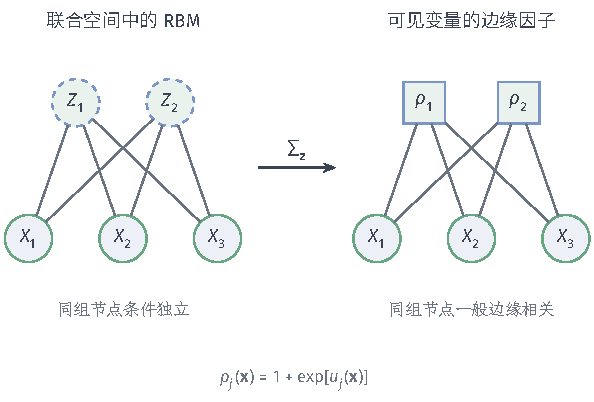
\includegraphics[width=\linewidth]{figures/03-models/03-probabilistic-graphical-models/tikz/pgm-energy-models-rbm/figure.pdf}
  \caption{左侧RBM只有可见组与隐藏组之间的边；固定任一组，另一组条件独立。右侧消去两个隐藏节点，每个方形因子代表$1+\exp[u_j(\bm{x})]$，均作用于三个可见变量。两侧均省略可见偏置对应的一元势。二部条件独立不等于可见变量边缘独立。}
  \label{fig:pgm-energy-models-rbm}
\end{figure}

考虑两个可见节点、一个隐藏节点，偏置全为零，$W_{1,1}=W_{2,1}=\log2$。则$e^{-F(\bm{x})}=1+2^{x_1+x_2}$，按$(0,0),(0,1),(1,0),(1,1)$排列的权重为$2,3,3,5$，配分函数为$13$。给定$(x_1,x_2)=(1,1)$，隐藏节点为$1$的概率是$4/5$；给定$z=0$，两个可见节点独立且各以$1/2$的概率为$1$，给定$z=1$则各以$2/3$的概率为$1$。边缘上却有$p(X_1=X_2=1)=5/13$，而$p(X_1=1)p(X_2=1)=(8/13)^2$，二者相差$1/169$。

计算一个自由能只需$O(d_{\mathrm{v}}m)$运算，但$Z_{\bm{\theta}}=\sum_{\bm{x}}e^{-F_{\bm{\theta}}(\bm{x})}$一般仍需指数级求和。利用两侧的条件分解，可枚举较小的一组并解析消去另一组，但代价仍含$2^{\min(d_{\mathrm{v}},m)}$。因此，RBM解决了给定完整可见向量的隐藏后验计算，没有一般地解决联合归一化；若部分可见变量缺失，求$p(\bm{z}\mid\bm{x}_{\mathrm{obs}})$也不再直接是上述独立Bernoulli乘积。

二部结构适合\term{交替Gibbs采样}（alternating Gibbs sampling）：轮流固定一组，独立抽取另一组。算法~\ref{alg:pgm-energy-models-rbm-gibbs}中的抽取必须使用随机二值状态；把概率直接作为下一层的输入会变成另一种迭代，不再是这个Gibbs核。

\begin{algorithm}[RBM的一段交替Gibbs链]
  \label{alg:pgm-energy-models-rbm-gibbs}
  \begin{algorithmic}[1]
    \Require 固定的有限参数$\bm{\theta}$，初始状态$\bm{x}^{(0)}$，步数$k\geq1$
    \Ensure 链状态$\bm{x}^{(1)},\ldots,\bm{x}^{(k)}$
    \For{$t=0,\ldots,k-1$}
      \State 按式~\eqref{eq:pgm-energy-models-rbm-conditionals}独立抽取各$Z_j^{(t+1)}$
      \State 固定$\bm{z}^{(t+1)}$，独立抽取各$X_i^{(t+1)}$
    \EndFor
  \end{algorithmic}
\end{algorithm}

固定有限参数时，所有条件概率都严格介于$0$与$1$，该有限状态链能够到达任意可见配置且存在自转移，并保持$p_{\bm{\theta}}(\bm{x})$不变。由第~\ref{chap:pgm-sampling}章的有限链理论可得长期收敛，但不能据此保证小$k$已充分混合。一次完整更新为$O(d_{\mathrm{v}}m)$；强权重造成的近确定条件分布会使链长时间停留在少数模式。

将第~\ref{chap:pgm-parameter-learning}章的潜变量似然梯度实例化到一个权重，单条数据$\bm{x}$给出
\begin{equation}
  \frac{\partial\log p_{\bm{\theta}}(\bm{x})}
       {\partial W_{i,j}}
    =x_i\,p_{\bm{\theta}}(Z_j=1\mid\bm{x})
      -\mathbb{E}_{p_{\bm{\theta}}}[X_iZ_j].
  \label{eq:pgm-energy-models-rbm-gradient}
\end{equation}
第一项可以精确计算，第二项通常由采样估计。多条记录对第一项取样本平均，偏置更新则使用相应的一阶统计量。RBM的训练收益来自前一项的简化，不来自后一项的消失。短链重构误差小也不是模型似然高的证据：混合很慢的链可能总能留在起始数据附近，却没有正确表达不同模式之间的概率质量\scite{pgm-energy-models-hinton2010}

图~\ref{fig:rbm-alternating-sampling-and-gradient}将条件概率、抽到的状态与训练统计分开。链内参数保持固定，交替抽样用来估计模型统计，随后才由数据统计与模型统计之差更新参数。

\begin{figure*}[htbp]
  \centering
  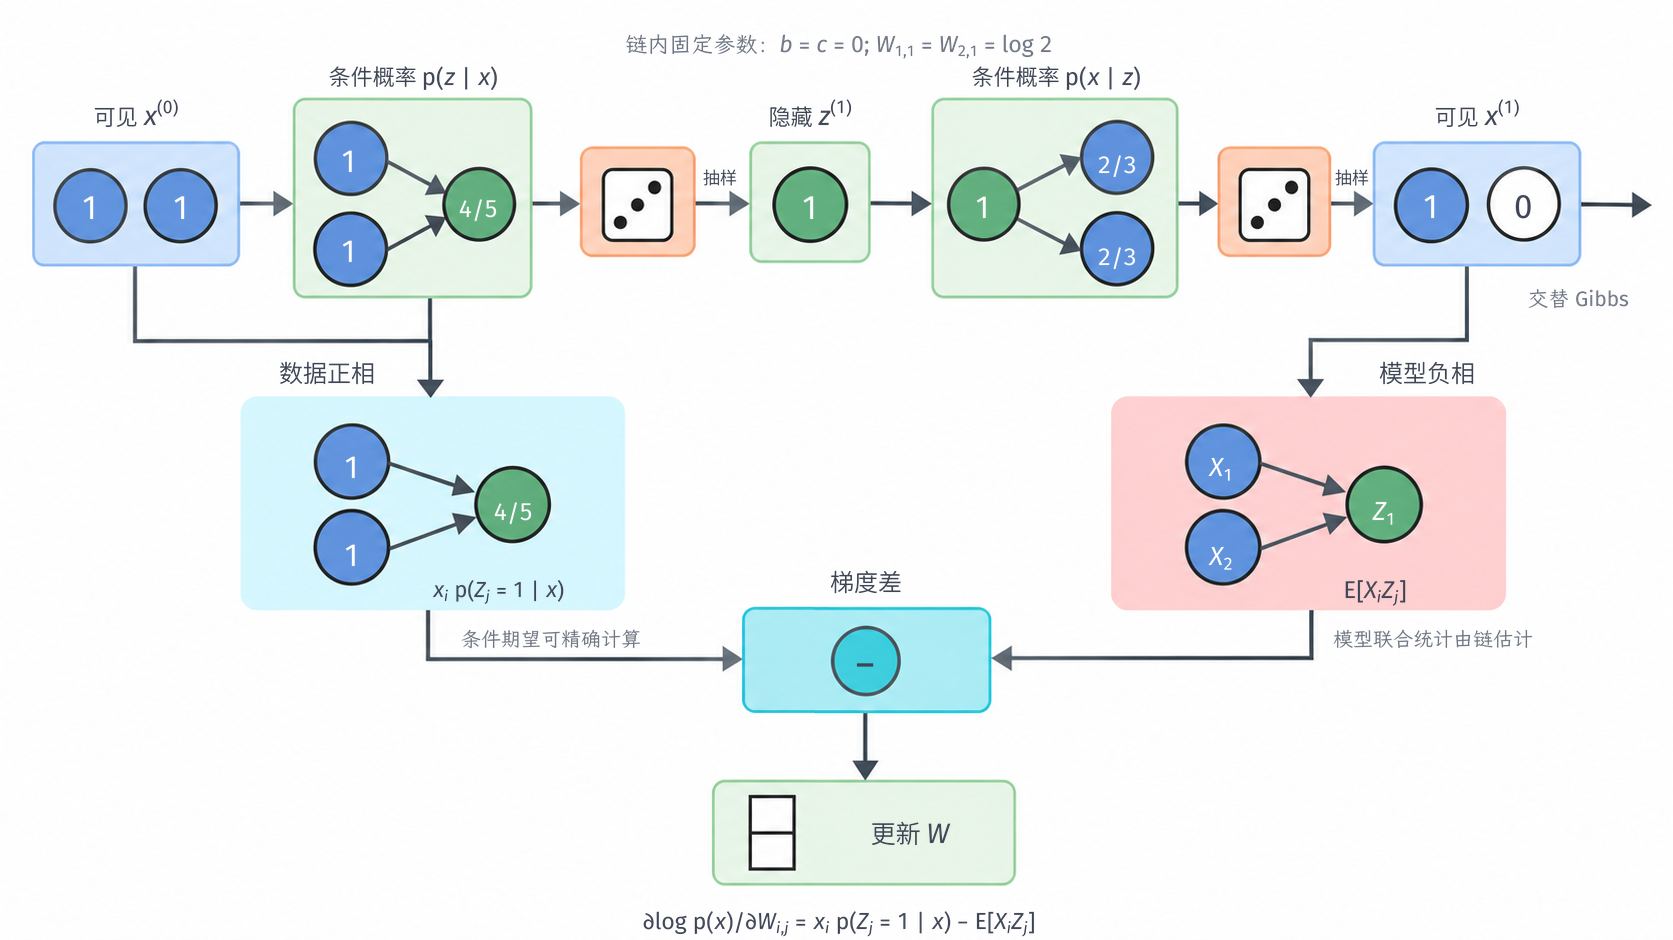
\includegraphics[width=\linewidth]{figures/03-models/03-probabilistic-graphical-models/generated/rbm-alternating-sampling-and-gradient/figure.png}
  \caption{二值RBM的交替抽样与似然梯度。固定$b=c=0$、$W_{1,1}=W_{2,1}=\log2$；可见状态$(1,1)$给出隐藏条件概率$4/5$，若抽到$z=1$，两可见单元的条件概率均为$2/3$，随后可能抽到$(1,0)$。条件概率与随机状态分开显示。权重梯度为可精确计算的数据统计减去模型联合统计，后者由链估计；单步重构不表示链已混合。}
  \label{fig:rbm-alternating-sampling-and-gradient}
\end{figure*}

\subsection{灵活能量模型}
\label{sec:pgm-energy-models-flexible}

二次能量与二值成对能量把相互作用限制在较简单的函数形式中。若数据中的相容关系需要更复杂的非线性特征，可以用神经网络输出一个标量能量。\term{神经能量模型}（neural energy-based model）仍由$p_{\bm{\theta}}(\bm{x})\propto e^{-E_{\bm{\theta}}(\bm{x})}$定义，只是用网络参数控制哪些配置具有低能量。网络中的确定性隐藏激活不是自动需要边缘化的随机潜变量；是否存在潜变量，要看概率模型是否为它们定义了分布。

若保留局部分解$E_{\bm{\theta}}(\bm{x})=\sum_CE_{\bm{\theta},C}(\bm{x}_C)$，可以让每个局部网络表示复杂势，同时保留既定图的独立性承诺。若一个网络同时读取所有$x_i$且没有额外分解，它可能形成全局高阶势，不能再仅凭网络内部连接图声称数据变量有稀疏Markov结构。神经参数化扩大了函数族，并没有自动带来较低的推断宽度。

连续模型还须控制尾部。一个容易验证的充分条件是
\[
  E_{\bm{\theta}}(\bm{x})
    =\frac{\alpha}{2}\lVert\bm{x}\rVert_2^2+r_{\bm{\theta}}(\bm{x}),
  \qquad \alpha>0,\quad r_{\bm{\theta}}(\bm{x})\geq-C,
\]
其中$C$有限、能量可测且在正测度集合上有限。此时$e^{-E_{\bm{\theta}}(\bm{x})}\leq e^Ce^{-\alpha\lVert\bm{x}\rVert_2^2/2}$，由高斯积分可知$0<Z_{\bm{\theta}}<\infty$。这是一个充分条件，不是任意神经网络天然满足的性质。把支持限制在有限体积区域并使能量有适当下界，也是另一种明确的建模选择。

分类网络的得分则未必定义联合密度。对有限标签集合，把$s_k(\bm{x})$在$k$上做softmax，可得$p(Y=k\mid\bm{x})$；给所有$s_k$同时加上任意$c(\bm{x})$，条件概率不变，但$\sum_ke^{s_k(\bm{x})}$会随之改变。因此，仅有分类训练不能唯一确定输入密度，更不能直接把某个得分称为$\log p(\bm{x})$。采用能量形式时，必须同时说明支持、归一化对象及训练准则。

神经能量通常没有RBM那样的解析块条件分布。在无约束的$\mathbb{R}^d$上，对连续可微能量可用数据空间梯度驱动采样，例如Langevin离散更新
\begin{equation}
  \begin{aligned}
    \bm{x}^{(t+1)}
      &=\bm{x}^{(t)}
        -\frac{\varepsilon}{2}
          \nabla_{\bm{x}}E_{\bm{\theta}}(\bm{x}^{(t)})
        +\sqrt{\varepsilon}\,\bm{\xi}^{(t)},\\
    \bm{\xi}^{(t)}&\sim\mathcal{N}(\bm{0},\bm{I}),
       \qquad \varepsilon>0.
  \end{aligned}
  \label{eq:pgm-energy-models-langevin}
\end{equation}
独立高斯噪声让状态不仅沿能量下降，也能够探索邻近区域。未经Metropolis校正的固定步长离散链一般有偏差，其稳定性还需要对能量梯度施加条件；有限步链也有初始化与混合误差。若一次能量梯度求值的成本为$C_E$，每条$k$步负样本链的梯度计算成本为$O(kC_E)$，不能把一次网络前向传播的成本当作生成一个样本的全部成本。连续神经能量结合梯度采样的具体实现可见Du与Mordatch的工作，其有限步训练程序不应被解释为任意能量下的精确采样保证\scite{pgm-energy-models-du2019}

训练时，对比散度从数据启动短链，以链终点近似模型期望；持久链保留上轮状态，尝试跟踪随参数缓慢变化的模型。这两种做法改变的是模型期望的取得方式，不保证有限步更新等于精确似然梯度。对神经能量，偏差还会反过来影响正在学习的能量形状；训练若只见到某些局部区域的负样本，其他区域可能出现未被约束的低能量值。上述性质及对比散度并非一般固定目标精确梯度的原因，见第~\ref{chap:pgm-parameter-learning}章。

噪声对比估计不需要每轮运行模型链，而以已知噪声分布$p_{\mathrm{N}}$构造分类任务；这里使用的对数比为$-E_{\bm{\theta}}(\bm{x})+c-\log[\nu p_{\mathrm{N}}(\bm{x})]$，$\nu$为噪声与数据样本数量比，$c$作为全局归一化参数学习。它不同于随意训练一个数据分类器：噪声密度和样本比例明确进入目标，且噪声必须覆盖相关支持。高维噪声若与数据过易区分，分类信号未必足以精细调整数据附近的密度。

对光滑连续密度，分数匹配利用$\nabla_{\bm{x}}\log p_{\bm{\theta}}=-\nabla_{\bm{x}}E_{\bm{\theta}}$消去配分函数。在式~\eqref{eq:pgm-parameter-learning-score-matching}所说明的可积性与零边界项条件下，其可优化部分写成
\[
  \mathbb{E}_{p_*}\!\left[
      \frac12\lVert\nabla_{\bm{x}}E_{\bm{\theta}}(\bm{X})\rVert_2^2
      -\Delta_{\bm{x}}E_{\bm{\theta}}(\bm{X})\right],
\]
其中$p_*$是数据分布，$\Delta_{\bm{x}}$为各坐标二阶偏导之和。代价转向输入导数，尤其是高维Hessian迹的计算或估计。标准形式既不直接适用于离散状态，也不能忽略受限支持的边界项；它避免训练时的归一化计算，却没有使最终的$Z$变成已知。结合加噪数据的分数学习将在第~\ref{chap:pgm-generative}章继续讨论。

\subsection{高阶与关系联合模型}
\label{sec:pgm-energy-models-higher-relational}

有些约束针对一组节点的整体状态，而非逐对相容性。例如，一组传感器中恰有一个应被激活，或一个逻辑条件同时涉及设备、连接关系和报警。\term{高阶势}（higher-order potential）让三个或更多变量共同决定一个局部权重。对二值节点，令$k_C=\sum_{i\in C}\mathbf{1}\{x_i=+1\}$，能量$g(k_C)$可表达计数偏好；$\lambda\mathbf{1}\{k_C\ne k_0\}$惩罚计数不等于$k_0$，$\lambda\mathbf{1}\{0<k_C<|C|\}$则惩罚组内不一致，其中$\lambda>0$、$k_0\in\{0,\ldots,|C|\}$。

作用域大并不必然意味着存在不可约的高阶相互作用。例如，平方计数代价$(k_C-k_0)^2$展开后只含常数、一元项和成对项。要看真正的区别，可取三个$\{-1,+1\}$变量，令$p(\bm{x})\propto\exp(\lambda x_1x_2x_3)$，$\lambda\ne0$。这个模型奖励某种乘积符号，且
\[
  \sum_{\bm{x}\in\{-1,+1\}^3}
     x_1x_2x_3\log p(\bm{x})=8\lambda.
\]
常数归一化项乘以$x_1x_2x_3$求和为零，剩余项为八个$\lambda$。若同一正分布能够只由这三个变量上的一元和成对势表示，对任一局部对数势，总有一个不在其作用域内的变量，先对该变量求和便得零，因此左侧必须为零，产生矛盾。这证明了该分布不能在不引入额外变量的前提下改写成成对模型；它不排除引入潜变量后的其他表示。

推断的成本取决于高阶势是否还有可利用的代数结构。对$r$个二值变量的任意稠密因子，一张表有$2^r$个条目，向一个变量计算消息一般要遍历其他$2^{r-1}$种配置。纯计数势则可先用动态规划累加其余节点“恰有$k$个为$+1$”的加权总量，再乘上对应的$e^{-g(k)}$求和；单个输出消息的计数卷积可在$O(r^2)$时间内完成。这个局部简化不会消除其他因子引起的全局环。学习时，计数区间的指示量或整体一致性指标替代成对统计量，梯度仍由相应经验值与模型期望之差组成。

当同一种约束要在许多实体上重复使用，逐个手写因子既冗长又容易不一致。\term{关系模板}（relational template）规定“哪些类型的实体及关系组成一个因子，以及这些因子共用哪些参数”。把模板中的实体占位符替换为具体对象，称为\term{落地}（grounding）；得到的仍是普通图模型，但节点和因子可能非常多。参数共享只压缩参数数量，不会使落地实例彼此独立。

\term{Markov逻辑网络}（Markov logic network, MLN）把逻辑公式作为这种模板，并按公式成立的落地次数为联合配置计分。为保证对象明确，这里取有限实体域$D$、有限个谓词，不允许产生无限项的函数符号；考虑带有自由实体变量、按所有域元素替换的公式模板。每个落地原子命题对应一个Boolean随机变量，所有命题真值组成一个配置$\bm{x}$。若模板$r$的权重为$w_r$、落地集合为$\mathcal{I}_r(D)$，则
\begin{equation}
  \begin{aligned}
    n_r(\bm{x})
      &=\sum_{g\in\mathcal{I}_r(D)}
           \mathbf{1}\{\text{公式 }r\text{ 在落地 }g\text{ 上为真}\},\\
    E_{\bm{\theta}}(\bm{x})&=-\sum_rw_rn_r(\bm{x}),\\
    p_{\bm{\theta}}(\bm{x})
      &=Z_{\bm{\theta}}^{-1}
          \exp\!\left[\sum_rw_rn_r(\bm{x})\right].
  \end{aligned}
  \label{eq:pgm-energy-models-mln}
\end{equation}
公式内部的逻辑蕴含不是有向概率边。正权重表示满足该公式的配置得到奖励，并不要求每个实例都满足公式；有限权重下允许矛盾实例以非零概率出现。

例如，$\operatorname{Fault}(a)\Rightarrow\operatorname{Alarm}(a)$把同一设备的两种命题联系起来。另一个模板
\[
  \operatorname{Linked}(a,b)\land\operatorname{Fault}(a)
       \ \Rightarrow\ \operatorname{Fault}(b)
\]
还涉及不同设备及其连接关系。落地$(a,b)=(u,v)$时，三个原子命题共同进入一个因子；若连接关系也是未知变量，因子便是三阶的。图中两节点相连，是因为相应命题共同出现在某个落地公式中，而不是因为两个实体之间必然有物理连接。固定连接证据以后，因子可能简化，但这属于对原联合模型的条件化。

权重也不能直接读成规则正确率。只取一个设备的第一个模板，设$w=\log4$且没有其他势，将故障与报警命题的真值分别记为$F,A$。按$(F,A)=(0,0),(0,1),(1,0),(1,1)$排列，逻辑蕴含为真的三个配置权重均为$4$，唯一违反配置$(1,0)$的权重为$1$，所以$Z=13$。公式成立的概率是$12/13$，而$p(A=1\mid F=1)=4/5$、$p(A=1)=8/13$。这些都是同一模型的不同查询，没有一个可被不加条件地称为权重对应的“规则概率”。引入其他重叠公式以后，条件概率还会随周围命题的证据改变。

MLN的似然学习比较观测世界中的$n_r$与模型预期的$n_r$，一个参数的梯度汇总该模板的所有落地实例。完整世界可用伪似然避开联合配分函数；只观测部分命题时，数据相关统计量本身也需要后验推断。推断则可以在相关落地图上消元、传递近似消息或采样。含$q$个实体占位符的模板在大小为$N=|D|$的域上可能产生$O(N^q)$个实例，精确推断还受落地图宽度限制；不能以模板很短推断计算很轻。MLN的定义、落地与伪似然学习见Richardson和Domingos的原始工作\scite{pgm-energy-models-richardson2006}

把规则设为硬约束相当于排除违反配置，但约束矛盾时可能使$Z=0$，硬约束还可能让单点采样无法穿越不同可行区域。即使全部采用软约束，扩大实体域也会改变落地次数及不同模板的相对影响；直接复用权重不保证保留原域中的边缘概率。因此，关系共享解决的是重复结构的表达与统计合并，不是自动保证跨域规模的概率一致性。

\section{条件能量模型}
\label{sec:pgm-energy-models-conditional-models}

在检测任务中，输入常包含温度、历史窗口摘要和传感器类型等已知信息。若只需据此输出一组异常标签，为这些输入建立精确联合分布可能超出了任务所需。条件能量模型固定输入，把表示和计算资源集中到标签之间的相容关系上；它仍需要全局比较输出配置，而不是把每个标签独立分类。

\subsection{条件随机场的定义}
\label{sec:pgm-energy-models-crf-definition}

\term{条件随机场}（conditional random field, CRF）是给定输入以后、输出变量按照某个无向图满足Markov性质的条件分布。实际建模通常直接给出输入相关的团势：
\begin{equation}
  \begin{aligned}
    p_{\bm{\theta}}(\bm{y}\mid\bm{x})
      &=\frac{1}{Z_{\bm{\theta}}(\bm{x})}
          \prod_{C\in\mathcal{C}}
             \psi_{\bm{\theta},C}(\bm{y}_C,\bm{x}),\\
    E_{\bm{\theta}}(\bm{y},\bm{x})
      &=-\sum_{C\in\mathcal{C}}
             \log\psi_{\bm{\theta},C}(\bm{y}_C,\bm{x}).
  \end{aligned}
  \label{eq:pgm-energy-models-crf-factors}
\end{equation}
图的节点对应输出变量；在固定输入下，若$S$分离$A$与$B$，则$\bm{Y}_A\perp\bm{Y}_B\mid(\bm{Y}_S,\bm{x})$。输入可以进入多个势，也可以被完整序列编码器处理；只有一个势同时依赖哪些未知标签，才直接决定此处的标签作用域。

对一个既定联合Markov网络$p(\bm{x},\bm{y})$进行条件化，也会得到这种形式，但这与直接拟合条件分布不是相同的学习任务。联合学习还约束$p(\bm{x})$，直接条件学习则没有这项要求。反过来，在给定一个CRF后可以另选$p(\bm{x})$组成联合分布，但这个额外选择并非CRF本身确定。对缺失输入求概率边缘同样需要额外的输入模型，不能直接从$p(\bm{y}\mid\bm{x})$中完成。

在常用线性参数化中，$\log\psi_{\bm{\theta},C}=\bm{\theta}^\top\bm{f}_C(\bm{x},\bm{y}_C)$，不同作用域可共用参数。对完整标签记录$\{(\bm{x}_r,\bm{y}_r)\}_{r=1}^n$，条件对数似然为
\begin{equation}
  \ell_{\mathrm{cond}}(\bm{\theta})
    =\sum_{r=1}^n
       \left[
        \sum_C\bm{\theta}^\top
                    \bm{f}_C(\bm{x}_r,\bm{y}_{r,C})
        -\log Z_{\bm{\theta}}(\bm{x}_r)
       \right].
  \label{eq:pgm-energy-models-crf-likelihood}
\end{equation}
每条输入通常对应不同的配分函数。梯度需要每条输入下的标签边缘，以计算期望特征；精确推断因此既用于预测，也反复出现在训练中。固定特征、完整标签、线性参数化时该对数似然是凹的，但有限最优解的存在仍需考虑可分离性和正则化；使用可训练神经特征或边缘化未观测标签后，不能沿用一般凹性结论。梯度推导见第~\ref{sec:pgm-parameter-learning-conditional}节，CRF的系统表述可参见Sutton与McCallum\scite{pgm-energy-models-sutton2012}

\subsection{线性链条件随机场}
\label{sec:pgm-energy-models-linear-chain}

若标签对应按顺序排列的位置，且每个标签只与相邻标签直接相互作用，可以保留链状输出图。\term{线性链条件随机场}（linear-chain CRF）把得分拆为状态项和转移项。令序列长度为$T$，$y_t\in\{1,\ldots,K\}$，有
\begin{equation}
  \begin{aligned}
    f_{\bm{\theta}}(\bm{y},\bm{x})
      &=\sum_{t=1}^T a_t(y_t;\bm{x})
        +\sum_{t=2}^T b_t(y_{t-1},y_t;\bm{x}),\\
    p_{\bm{\theta}}(\bm{y}\mid\bm{x})
      &\propto e^{f_{\bm{\theta}}(\bm{y},\bm{x})}.
  \end{aligned}
  \label{eq:pgm-energy-models-chain-score}
\end{equation}
$a_t$评价输入与当前位置标签的相容性，$b_t$评价相邻标签组合；记$\phi_t(k)=e^{a_t(k;\bm{x})}$、$\psi_t(j,k)=e^{b_t(j,k;\bm{x})}$，参数依赖暂略。始末状态偏好可并入$a_1$和$a_T$。这里的“转移”是相邻标签的势，不要求$\sum_k\psi_t(j,k)=1$，也不指定因果生成顺序。

链的分解允许把指数多条前缀合并。\term{前向消息}（forward message）$\alpha_t(k)$是所有以$y_t=k$结尾的长度$t$前缀的未归一化权重和。把每个前缀按倒数第二个标签分组，有
\begin{equation}
  \begin{aligned}
    \alpha_1(k)&=\phi_1(k),\\
    \alpha_t(k)&=\phi_t(k)
       \sum_{j=1}^K\alpha_{t-1}(j)\psi_t(j,k),
       \qquad t=2,\ldots,T,\\
    Z_{\bm{\theta}}(\bm{x})&=\sum_{k=1}^K\alpha_T(k).
  \end{aligned}
  \label{eq:pgm-energy-models-forward}
\end{equation}
该递推没有省略任何序列：任一长度$t$的标签前缀恰好属于一个末标签对$(j,k)$，其权重是旧前缀权重乘上新增状态势与边势。对$t$作归纳便证明$\alpha_t$的定义始终成立。

为了计算中间位置的边缘，还需汇总右侧信息。定义$\beta_t(j)$为固定$y_t=j$以后、从$t+1$到$T$的后缀权重和，不含当前位置状态势，则
\begin{equation}
  \begin{aligned}
    \beta_T(j)&=1,\\
    \beta_t(j)&=\sum_{k=1}^K
         \psi_{t+1}(j,k)\phi_{t+1}(k)\beta_{t+1}(k),\\
    p(Y_t=k\mid\bm{x})
      &=\frac{\alpha_t(k)\beta_t(k)}{Z_{\bm{\theta}}(\bm{x})}.
  \end{aligned}
  \label{eq:pgm-energy-models-backward}
\end{equation}
固定相邻标签后，左右两段也分别分解，因此
\begin{equation}
  p(Y_{t-1}=j,Y_t=k\mid\bm{x})
   =\frac{\alpha_{t-1}(j)\psi_t(j,k)
                   \phi_t(k)\beta_t(k)}
          {Z_{\bm{\theta}}(\bm{x})}.
  \label{eq:pgm-energy-models-edge-marginal}
\end{equation}
状态边缘与边边缘恰好足以计算式~\eqref{eq:pgm-energy-models-chain-score}中局部特征的模型期望；求和消元的通用原理见第~\ref{chap:pgm-elimination}章。

现在沿用三位置例子，把未知状态改记为标签$y_t\in\{-1,+1\}$。边势仍在同号时为$3$、异号时为$1$；某个固定输入给出的状态势，按$(-1,+1)$排列，三个位置分别取$(1,2)$、$(1,1)$、$(1,3)$。输入偏好首尾为正，中间位置没有局部偏好。表~\ref{tab:pgm-energy-models-chain-weights}列出全部配置，使归一化和解码都可直接核验。

\begin{table}[htbp]
  \centering
  \begin{tabular}{crr}
    \toprule
    状态或标签配置 & 联合权重$w_0$ & 条件权重$w_{\bm{x}}$\\
    \midrule
    $(-,-,-)$ & $9$ & $9$\\
    $(-,-,+)$ & $3$ & $9$\\
    $(-,+,-)$ & $1$ & $1$\\
    $(-,+,+)$ & $3$ & $9$\\
    $(+,-,-)$ & $3$ & $6$\\
    $(+,-,+)$ & $1$ & $6$\\
    $(+,+,-)$ & $3$ & $6$\\
    $(+,+,+)$ & $9$ & $54$\\
    \midrule
    总和 & $32$ & $100$\\
    \bottomrule
  \end{tabular}
  \caption{同一组相邻势下的联合与条件权重。符号$+$、$-$分别表示$+1$、$-1$；条件列在联合列上乘以固定输入给出的三项状态势。两列须分别除以各自总和，不能把状态势误当作已归一化的标签概率。}
  \label{tab:pgm-energy-models-chain-weights}
\end{table}

把两个标签对应的消息值按$(-1,+1)$组成向量，前向递推给出$\bm{\alpha}_1=(1,2)$、$\bm{\alpha}_2=(5,7)$、$\bm{\alpha}_3=(22,78)$，例如$\alpha_2(+1)=1(1\times1+2\times3)=7$。因此$Z(\bm{x})=100$。后向递推给出$\bm{\beta}_3=(1,1)$、$\bm{\beta}_2=(6,10)$、$\bm{\beta}_1=(28,36)$，所以
\[
  p(Y_2=+1\mid\bm{x})=\frac{7\times10}{100}=0.7.
\]
中间位置没有自己的类别偏好，却从两侧输入获得了正类证据。两条边同号的边缘概率都为$0.78$；若训练标签是$(+,+,+)$，共享的同号得分参数$\eta=\log3$在该记录上的似然梯度就是$2-2\times0.78=0.44$，推动模型增加同号序列的相对权重。这里仅实例化期望特征，并未将不同边视为独立训练记录。

如果任务是找最可能的完整标签序列，则应把前向求和换成取最大，并保存前驱。这是\term{Viterbi算法}（Viterbi algorithm），即在链上复用最优前缀的动态规划。用对数得分避免连乘，有
\begin{equation}
  \begin{aligned}
    \delta_1(k)&=a_1(k;\bm{x}),\\
    \delta_t(k)&=a_t(k;\bm{x})
       +\max_j\{\delta_{t-1}(j)+b_t(j,k;\bm{x})\}.
  \end{aligned}
  \label{eq:pgm-energy-models-viterbi}
\end{equation}
对每个$(t,k)$保存达到最大值的$j$，从$\argmax_k\delta_T(k)$向前回溯；平局可按固定标签顺序选择一个最优解。在数值例子中，将$\exp[\delta_t(k)]$按标签$(-1,+1)$排列，三步依次为$(1,2),(3,6),(9,54)$，回溯得到$(+,+,+)$，概率为$0.54$。逐位置选择边缘最大的标签优化的是逐位置错误的期望，不是完整序列概率；本例二者恰好相同，不能据此将两种解码等同。最大积也只适用于这里对全部未知标签的联合最大化；若另有潜变量要先求和，需重新区分联合最优与边缘MAP。

前向、后向和Viterbi各需要$O(TK^2)$时间。仅求配分函数时消息空间为$O(K)$，保留全部节点边缘或解码回溯通常需要$O(TK)$消息或前驱空间；若存储所有稠密边势，另需$O(TK^2)$空间。长序列应使用对数域的log-sum-exp，或逐步缩放并记录缩放常数，否则数值下溢会破坏归一化。每条训练记录的梯度也需要同量级的前向后向推断，特征提取或神经编码器的成本另计。

输入的远程信息可以进入$a_t$，而不改变上述标签递推；直接加入$y_t$与远处未知标签的耦合则会改变图结构。线性链适合局部标签依赖，但不能独立表达任意长程标签约束。与局部归一化的逐状态分类器相比，CRF让整个输出序列共同竞争概率质量；代价是每次训练与概率查询都要处理完整链的归一化，而不是分别拟合各个状态的分类概率\scite{pgm-energy-models-sutton2012}

\subsection{半Markov与高阶条件随机场}
\label{sec:pgm-energy-models-semi-higher}

有些输出对象本来就是片段：一个异常区间的长度、区间内部温度的整体形状，都难以只用相邻标签对评价。\term{半Markov条件随机场}（semi-Markov CRF）将基本输出单位改为带标签的连续片段，让一个势同时评价片段的起止位置、整体输入及相邻片段标签。它仍对全部合法分段作一次条件归一化，不是先确定边界再各自分类。

设一次分段为$\bm{s}=((a_\ell,b_\ell,k_\ell))_{\ell=1}^M$，片段无重叠、无空隙地覆盖$1,\ldots,T$，即$a_1=1$、$a_{\ell+1}=b_\ell+1$、$b_M=T$，长度满足$1\leq b_\ell-a_\ell+1\leq L$。$k_\ell\in\{1,\ldots,K\}$是片段标签，$M$随分段变化；用$k_0=0$表示起始哨兵标签。令$g(a,b,j,k;\bm{x})$为前一片段标签$j$接上当前$[a,b]$、标签$k$的得分，则
\begin{equation}
  p_{\bm{\theta}}(\bm{s}\mid\bm{x})
   =\frac{\exp\!\left[
        \sum_{\ell=1}^M
          g(a_\ell,b_\ell,k_{\ell-1},k_\ell;\bm{x})
                    \right]}
          {Z_{\bm{\theta}}(\bm{x})}.
  \label{eq:pgm-energy-models-semi-distribution}
\end{equation}
配分函数对所有合法$\bm{s}$求和，包括不同边界和不同片段数。这里允许相邻片段有相同标签；若任务规定同标签相邻片段必须合并，就应把这项约束写入合法分段集合，算法也要禁止相应转移。

动态规划在片段边界处汇总信息。令$A_t(k)$为覆盖前$t$个位置且末片段标签为$k$的权重和，设$A_0(0)=1$、$A_0(k)=0$（$k>0$），并令$t>0$时$A_t(0)=0$。则
\begin{equation}
  A_t(k)=
    \sum_{\ell=1}^{\min(L,t)}\sum_{j=0}^K
       A_{t-\ell}(j)
       e^{g(t-\ell+1,t,j,k;\bm{x})}.
  \label{eq:pgm-energy-models-semi-forward}
\end{equation}
仅在首片段允许$j=0$。递推枚举末片段长度$\ell$和前一片段标签$j$，每个完整前缀都有唯一的这种拆分，因此没有重复计数；最终$Z(\bm{x})=\sum_{k=1}^KA_T(k)$。将求和改成最大并记录长度和标签，就能回溯最优分段。

学习片段特征还需要片段边缘。记$B_b(k)$为边界$b$之后、前一片段标签固定为$k$的所有后缀权重和，取$B_T(k)=1$，按下一片段的长度与标签反向递推即可。一次相邻片段连接的边缘概率为
\[
  \frac{A_{a-1}(j)
           e^{g(a,b,j,k;\bm{x})}B_b(k)}
       {Z_{\bm{\theta}}(\bm{x})}.
\]
这使长度、片段形状及片段转移等特征的期望可计算。若边界与片段标签全部已知，训练使用式~\eqref{eq:pgm-energy-models-semi-distribution}的对数概率；若只给定较粗标签、边界仍未知，分子也须对相容分段求和，不能拿一个最优分段代替这项边缘化。

一个极小例子可以核查“分段”与“逐点标签”的区别。取$T=3,K=1,L=2$，长度$1$片段的权重为$1$，长度$2$片段的权重为$2$，无其他得分。合法长度序列为$(1,1,1),(1,2),(2,1)$，权重分别为$1,2,2$。递推得到$A_1=1,A_2=3,A_3=5$，所以配分函数为$5$，位置$1$后出现边界的概率为$(1+2)/5=3/5$。所有分段都给出同一组逐点标签，但边界的不确定性仍然存在；长度上限排除的是一个长度$3$的单片段，不是三个同标签位置组成的序列。

若每个候选片段得分已可常数时间读取，一次前向或后向计算为$O(TLK^2)$，保存全部边界消息需要$O(TK)$空间；预先存储所有含转移的片段得分则可达$O(TLK^2)$。只求配分函数时可以滚动保留最近$L$个边界。若计算片段特征本身需要扫描片段内部，必须额外计入该成本。长度上限降低计算量，也会排除模型本来可能需要的长片段；不能仅因动态规划精确，就忽略候选集合的限制\scite{pgm-energy-models-sarawagi2004}

另一种扩展不改变逐点输出，而是扩大未知标签的作用域。\term{高阶条件随机场}（higher-order CRF）可以用$(r+1)$个连续标签共同决定一个势，即$E=-\sum_t f_t(y_{t-r},\ldots,y_t;\bm{x})$，序列起点使用固定哨兵补齐。在这种有限记忆结构下，消息需保留最近$r$个标签；每个位置有$K^r$种历史，每种历史接上$K$种新标签，所以朴素精确递推为$O(TK^{r+1})$时间、$O(K^r)$滚动消息空间。扩展状态间只能按共享后缀相接，不必建立任意$K^r\times K^r$稠密转移表。

图~\ref{fig:pgm-energy-models-crf-scopes}比较了这两种扩展。片段模型通过增加可选长度来表达持续区间；高阶链通过增加消息保留的标签组合来表达更长依赖。二者还可以组合，神经网络也可以参数化其中的局部得分，但其成本不能只用“一阶链”或“神经网络”的名称判断。若高阶势跨越任意远的未知标签，有限记忆递推也未必仍然适用。

\begin{figure}[htbp]
  \centering
  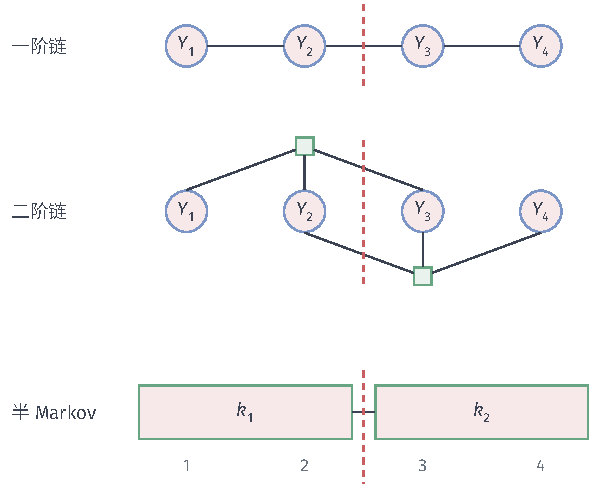
\includegraphics[width=\linewidth]{figures/03-models/03-probabilistic-graphical-models/tikz/pgm-energy-models-crf-scopes/figure.pdf}
  \caption{输出作用域的三种选择。一阶链的切分处只需保留一个标签；二阶链中，跨切分处的三元势需要保留两个标签。半Markov模型按片段边界递推，图中展示一种$[1,2]$与$[3,4]$的分段，推断时还须对其他合法边界求和。}
  \label{fig:pgm-energy-models-crf-scopes}
\end{figure}

\subsection{一般图与关系条件随机场}
\label{sec:pgm-energy-models-general-relational}

当输出对应二维检测网格，或分别属于存在连接关系的设备时，一条链无法保留所有必要相互作用。一般图CRF仍按式~\eqref{eq:pgm-energy-models-crf-factors}分解，但图由输出之间的关系决定。关系CRF进一步将这些作用域写成模板：已知设备属性、连接关系和图结构都进入输入，未知量则是待预测的标签。

例如，给每个设备一个标签$Y_i$，让设备属性产生一元势，让每条已知连接复用同一个相邻标签势。更一般地，若输入$\bm{x}$决定模板$r$的实例集合$\mathcal{I}_r(\bm{x})$，可写
\begin{equation}
  E_{\bm{\theta}}(\bm{y},\bm{x})
   =-\sum_r\sum_{g\in\mathcal{I}_r(\bm{x})}
        \bm{\theta}_r^\top
             \bm{f}_r(\bm{x}_g,\bm{y}_g).
  \label{eq:pgm-energy-models-relational-crf}
\end{equation}
这里$g$标识一组具体实体及关系所选出的作用域，$\bm{x}_g$是相关已知特征，$\bm{y}_g$是参与该因子的未知标签。同一个$\bm{\theta}_r$从全部实例汇总学习信号；不同实例可以重叠，不因此成为独立样本。Taskar等人的关系Markov网络工作给出了这类条件建模与集体分类的代表形式\scite{pgm-energy-models-taskar2002}

固定关系输入并没有自动使输出图无环。例如设备之间的连接形成一个闭环，标签势也会形成闭环。精确推断可以用第~\ref{chap:pgm-junction-tree}章的团树方法，复杂度由消元后的最大作用域决定。若每个标签有$K$种取值、所选消元序的诱导宽度为$w$，主要运算一般含$K^{w+1}$；简单环仍有较小宽度，并非出现一个环就必须近似。密集跨设备约束或大型高阶势则可能使团树不再可承受。

计算受限时，可以用第~\ref{chap:pgm-variational}章的平均场、环置信传播或最大化松弛，也可以用第~\ref{chap:pgm-sampling}章的采样。需要标签概率或条件似然梯度时，目标是边缘和期望；只需要完整标签的最优配置时，目标是最大化得分。对后者有效的图割或整数优化程序，不一定能返回前者。一般图上的环消息可能不收敛，即使收敛也不一般等于精确边缘；用其结果训练时，应明确正在使用近似梯度或近似配分函数。

关系模型还会放大建模假设的影响。若所有连接都被解释为“标签应相同”，实际连接却经常跨越不同故障类型，集体推断会把偏差传播到多个节点。度较大的节点参与更多势，局部错误也可能被多次计入；这需要在特征和参数共享方式上处理，不能靠扩大消息迭代次数修正。已知连接只是输入时，模型也没有定义未知连接的生成概率，不能直接把标签推断扩展成连接生成。

训练与评价应以任务中的完整关系结构为单位说明数据来源。在同一张大图上划分已标注与未标注节点可以构成合法的传导预测任务，但它不同于预测全新独立图；测试标签不得通过邻域特征进入训练。若只观测部分训练标签，需在条件似然分子中对其他标签求和，又会带来后验推断和通常非凹的优化。关系共享有助于合并重复模式的信息，不消除相关性、推断误差或划分泄漏。

\section{模型比较}
\label{sec:pgm-energy-models-comparison}

这些模型都把局部得分组合成全局概率，差别应落实到哪些变量参与归一化、哪些变量被观测，以及积分或求和能否利用结构。表~\ref{tab:pgm-energy-models-comparison}列出本章所讨论的代表设定；同一实例可以同时具有多行中的属性，例如神经高阶关系CRF仍然属于条件能量模型，不能把表中名称当作互斥分类。

\begin{table*}[htbp]
  \centering
  \small
  \begin{tabularx}{\linewidth}{p{27mm}p{19mm}p{24mm}p{24mm}X}
    \toprule
    代表设定 & 归一化对象 & 变量与潜变量 & 势的作用域 & 可计算性与主要限制\\
    \midrule
    Ising／Potts & 全部状态 & 离散；此处全观测 & 一元、成对 & 树上精确；一般图的全局求和与强耦合采样可能昂贵\\
    高斯MRF & 全部状态 & 连续；此处全观测 & 二次能量 & 正定精度下可解析归一化；矩阵填充与单峰限制\\
    BM／RBM & 可见与隐藏状态 & 二值；含潜变量 & 联合空间成对 & RBM的块条件与自由能可算，联合配分函数一般仍难\\
    神经联合能量 & 全部状态 & 可离散或连续；潜变量可选 & 局部或全局 & 网络求值不等于归一化；尾部、采样和学习偏差均需控制\\
    MLN & 落地命题配置 & Boolean；可有未观测命题 & 模板决定阶数 & 参数共享不消除落地数量及推断宽度的增长\\
    线性链CRF & 给定输入的标签 & 离散；此处完整标签 & 一元、相邻成对 & $O(TK^2)$精确归一化；不直接表示任意远程标签约束\\
    半Markov／高阶链CRF & 分段或标签组合 & 离散；边界可未观测 & 片段或连续高阶 & 分别受$L$与$K^r$影响；有限结构下可精确递推\\
    一般图关系CRF & 给定关系输入的标签 & 此处离散；标签可缺失 & 成对或高阶 & 低宽度可精确；宽图依赖近似推断且须重复用于学习\\
    \bottomrule
  \end{tabularx}
  \caption{按本章具体设定比较模型。$T$为序列长度，$K$为标签数，$L$为最大片段长度，$r$为高阶链保留的历史标签数。潜变量、势阶数与参数化方式可以组合；条件无向模型也可以有连续输出，此表不穷尽这些组合。}
  \label{tab:pgm-energy-models-comparison}
\end{table*}

联合与条件的选择主要由查询决定。若需要解释整组测量、补全不同类型的未知变量或生成新的联合配置，就需要相应联合模型；若始终固定输入，只评价标签预测，直接条件建模避免额外约束输入分布。条件化不等于局部归一化，也不保证计算更便宜：一个复杂的输出图仍可能难以求和，而且训练中每个不同输入都有自己的$Z_{\bm{\theta}}(\bm{x})$。

表示能力与计算代价也不能只靠“势是否成对”判断。GMRF即使有环也能借助二次结构计算，RBM即使只有成对边也可能难以归一化；计数高阶势可以利用卷积，任意高阶表却要付出指数存储。神经网络扩大局部函数族时可以保持原图，直接给全局配置打分则可能失去稀疏分解。真正相关的是运算的代数形式、未知变量作用域和消元后的宽度。

学习的主要障碍与这些推断结构对应。完整离散联合模型需要模型期望；BM还需要数据条件下的隐藏后验，RBM只简化了后者；连续神经能量常把计算预算花在生成负样本或求输入导数上。链式CRF虽可精确求期望，长序列、大标签集和大量样本仍使反复推断昂贵。判断一套训练流程时，应分别检查能量是否定义了合法分布、所需查询能否求出，以及近似训练究竟偏离了什么目标；这些问题不能用一个训练损失数值代替。

\section{本章小结}
\label{sec:pgm-energy-models-summary}

局部相容信息之所以能成为整组状态的概率，是因为所有配置的权重共同参与归一化。能量只是这些权重的负对数表示；绝对能量零点可以改变，状态之间的能量差以及归一化后的概率才决定模型行为。三位置例子中，未加输入时的配分函数为$32$；固定新的输入相关状态势后，标签配分函数变成$100$，中间位置即使没有自己的偏好，也会通过相邻作用获得两侧证据。

联合无向模型与条件无向模型区分的是求和对象，不是势是否复杂。引入潜变量可以把简单联合相互作用转成复杂边缘依赖，RBM的二部结构使隐藏后验和自由能可算，却未消除联合归一化。高阶势与关系模板可以表达整体约束，但须检查作用域、落地规模与硬约束的可行性。神经能量允许更灵活的函数形状，也需要单独保证可归一化并控制采样或替代学习准则的误差。

条件能量模型把输入视为给定，并不削弱对输出依赖的建模。链、片段和有限阶历史之所以可精确计算，是因为递推只需保留有限边界信息；一般输出图则仍受推断宽度限制。由此回到开篇的问题：是否需要解释测量的生成分布，决定选用联合无向模型还是条件无向模型；需要保留何种相互作用，以及能承受哪种求和或采样代价，决定其内部结构。模型选择、推断与参数学习必须在这两个层次上相互配合。

同样是序列结构，也可以先描述潜状态怎样演化，再描述观测怎样产生。第~\ref{chap:pgm-dynamic}章采用这一有向生成方式，继续使用链上的求和与最大化，但其局部因子是转移、发射分布，而非给定完整输入后的任意标签势。这一区别决定了模型能否直接预测未来观测。
